
%===========================================================
% do not change this formatting please :-)
%===========================================================
\documentclass[letter,12pt]{article}
\usepackage[margin=1in]{geometry}
\usepackage{pdfpages}
\usepackage{amssymb,amsmath,amsthm,mathrsfs,colortbl,fancyhdr,tcolorbox,enumitem}
\fancyhead{}
\fancyhead[L]{Collin McDevitt} %Replace "NAME: " WITH YOUR NAME
\fancyhead[C]{MATH 5235 HOMEWORK 01}
\fancyhead[R]{PAGE \thepage}
\fancyfoot{}
\renewcommand{\footrulewidth}{0.4pt}

\date{\today}
%===========================================================
% convenient commands -- feel free to add more as you see fit
%===========================================================
\newcommand{\C}{\mathbb{C}}
\newcommand{\K}{\mathbb{K}}
\newcommand{\Poly}{\mathcal{P}}
\newcommand{\Q}{\mathbb{Q}}
\newcommand{\R}{\mathbb{R}}
\newcommand{\dotp}{\boldsymbol{\cdot}}
\begin{document}
\pagestyle{fancy}
%===========================================================
%===========================================================
%===========================================================
% PROBLEM 1
%===========================================================
\begin{tcolorbox}
    \textbf{Problem 1.} For a fixed $a\in \mathbb{C}$, show that $\frac{|z-a|}{|1-\bar{a}z|}=1$ if $|z|=1$ and $1-\bar{a}z\not = 0$.

\end{tcolorbox}

\begin{proof}
    Assume $a\in \mathbb{C}$ and $z\in \mathbb{Z}$ with $|z|=1$ and $1-\bar{a}z\not = 0$. Then for some $x,y,c,d\in \mathbb{R}$ we have $a=x+iy$ and $z=c+id$. We also have $|z|=\sqrt{c^2+d^2}=1=c^2+d^2$

    Calculating $|1-\bar{a}z|$ yields \begin{align*}
        |1-\bar{a}z| & = |1-(x-iy)(c+id)|                                         \\
        |1-\bar{a}z| & = \sqrt{(1-xc-yd)^2+(yc-xd)^2}                             \\
        |1-\bar{a}z| & = \sqrt{1-2xc-2yd+2xcyd+x^2c^2+y^2d^2+y^2c^2-2ycxd+x^2d^2} \\
        |1-\bar{a}z| & =\sqrt{1-2xc-2yd+x^2c^2+x^2d^2+y^2d^2+y^2c^2}              \\
        |1-\bar{a}z| & =\sqrt{1-2xc-2yd+x^2(c^2+d^2)+y^2(c^2+d^2)}                \\
        |1-\bar{a}z| & =\sqrt{1-2xc-2yd+x^2+y^2}                                  \\
        |1-\bar{a}z| & =\sqrt{c^2+d^2+x^2+y^2-2xc-2yd}                            \\
        |1-\bar{a}z| & =\sqrt{(c-x)^2+(d-y)^2}                                    \\
        |1-\bar{a}z| & =|z-a|
    \end{align*}

    Based on the assumption of $|1-\bar{a}z|\not = 0$ we have $$\frac{|z-a|}{|1-\bar{a}z|}=1$$

\end{proof}

\begin{tcolorbox}
    \textbf{Problem 2.} For which $n$ is $i$ an $n$th root of unity?
\end{tcolorbox}
For any positive integer $n$ where $n\equiv 0\bmod 4$.

\begin{tabbing}

\end{tabbing}

\begin{tcolorbox}
    \textbf{Problem 3.} If the point $P$ on the sphere corresponds to $z$ under stereographic projection, show that the antipodal point $-P$ on the sphere corresponds to $-\frac{1}{\overline{z}}$.
\end{tcolorbox}

\begin{proof}
    Assume that the point $P$ corresponds to $z_0=x_0+iy_0$ under stereographic projection. Then solving for the point $z$ from the projection $-P$ by using the equations on page 12
    \[
        \begin{cases}
             & X=\frac{2x_0}{|z_0|^2+1}       \\
            \\
             & Y = \frac{2y_0}{|z_0|^2+1}     \\
            \\
             & Z= \frac{|z_0|^2-1}{|z_0|^2+1}
        \end{cases}
    \] substituting in for $z=-\frac{X}{1+Z}-i\frac{Y}{1+Z}$ we get
    \begin{align*}
        z & =-\frac{\frac{2x_0}{|z_0|^2+1}}{1+\frac{|z_0|^2-1}{|z_0|^2+1}}-i\frac{\frac{2y_0}{|z_0|^2+1}}{1+\frac{|z_0|^2-1}{|z_0|^2+1}} \\
        z & = -\frac{\frac{2x_0+i2y_0}{|z_0|^2+1}}{1+\frac{|z_0|^2-1}{|z_0|^2+1}}                                                        \\
        z & = -\frac{\frac{2x_0+i2y_0}{|z_0|^2+1}}{\frac{2|z_0|^2}{|z_0|^2+1}}
        \\
        z & = -\frac{x_0+iy_0}{|z_0|^2}                                                                                                  \\
        z & = -\frac{x_0+iy_0}{|z_0|^2}\cdot \frac{\frac{1}{z_0}}{\frac{1}{z_0}}                                                         \\
        z & = -\frac{1}{\bar{z_0}}
    \end{align*}



\end{proof}


\begin{tcolorbox}
    \textbf{Problem 4.} (a) Give a brief description of the function $z\mapsto w=z^3$, considered as a mapping from the $z$-plane to the $w$-plane. (b) Make branch cuts and define explicitly three branches of the inverse mapping.
\end{tcolorbox}
\begin{enumerate}[label=(\alph*)]
    \item As $z=\rho e^{i\theta_0}$ traces a ray from the origin then $w=\rho^3 e^{i3\theta}$ hence the angle is three times the angle of $z$ while $|w|=|z|^3$. As $z$ traverses a circle centred at the origin we have for every single loop $z$ completes $w$ completes $3$ in the same direction and the radius of the circle in the $w$-plane is $|w|=|z|^3$.
    \item The branch cut is $\mathbb{C}\setminus (-\infty , 0]$ and the three branches of the inverse mapping are $f_1(w)=|w|^{\frac{1}{3}}e^{i \frac{\text{Arg}w}{3}},w\in \mathbb{C}\setminus (-\infty,0]\\$$f_2(w)=|w|^{\frac{1}{3}}e^{i(\frac{\text{Arg}w}{3}+\frac{2\pi}{3})},w\in \mathbb{C}\setminus (-\infty,0]\\$ $f_3(w)=|w|^{\frac{1}{3}}e^{i(\frac{\text{Arg}w}{3}+\frac{4\pi}{3})},w\in \mathbb{C}\setminus (-\infty,0]$.
\end{enumerate}


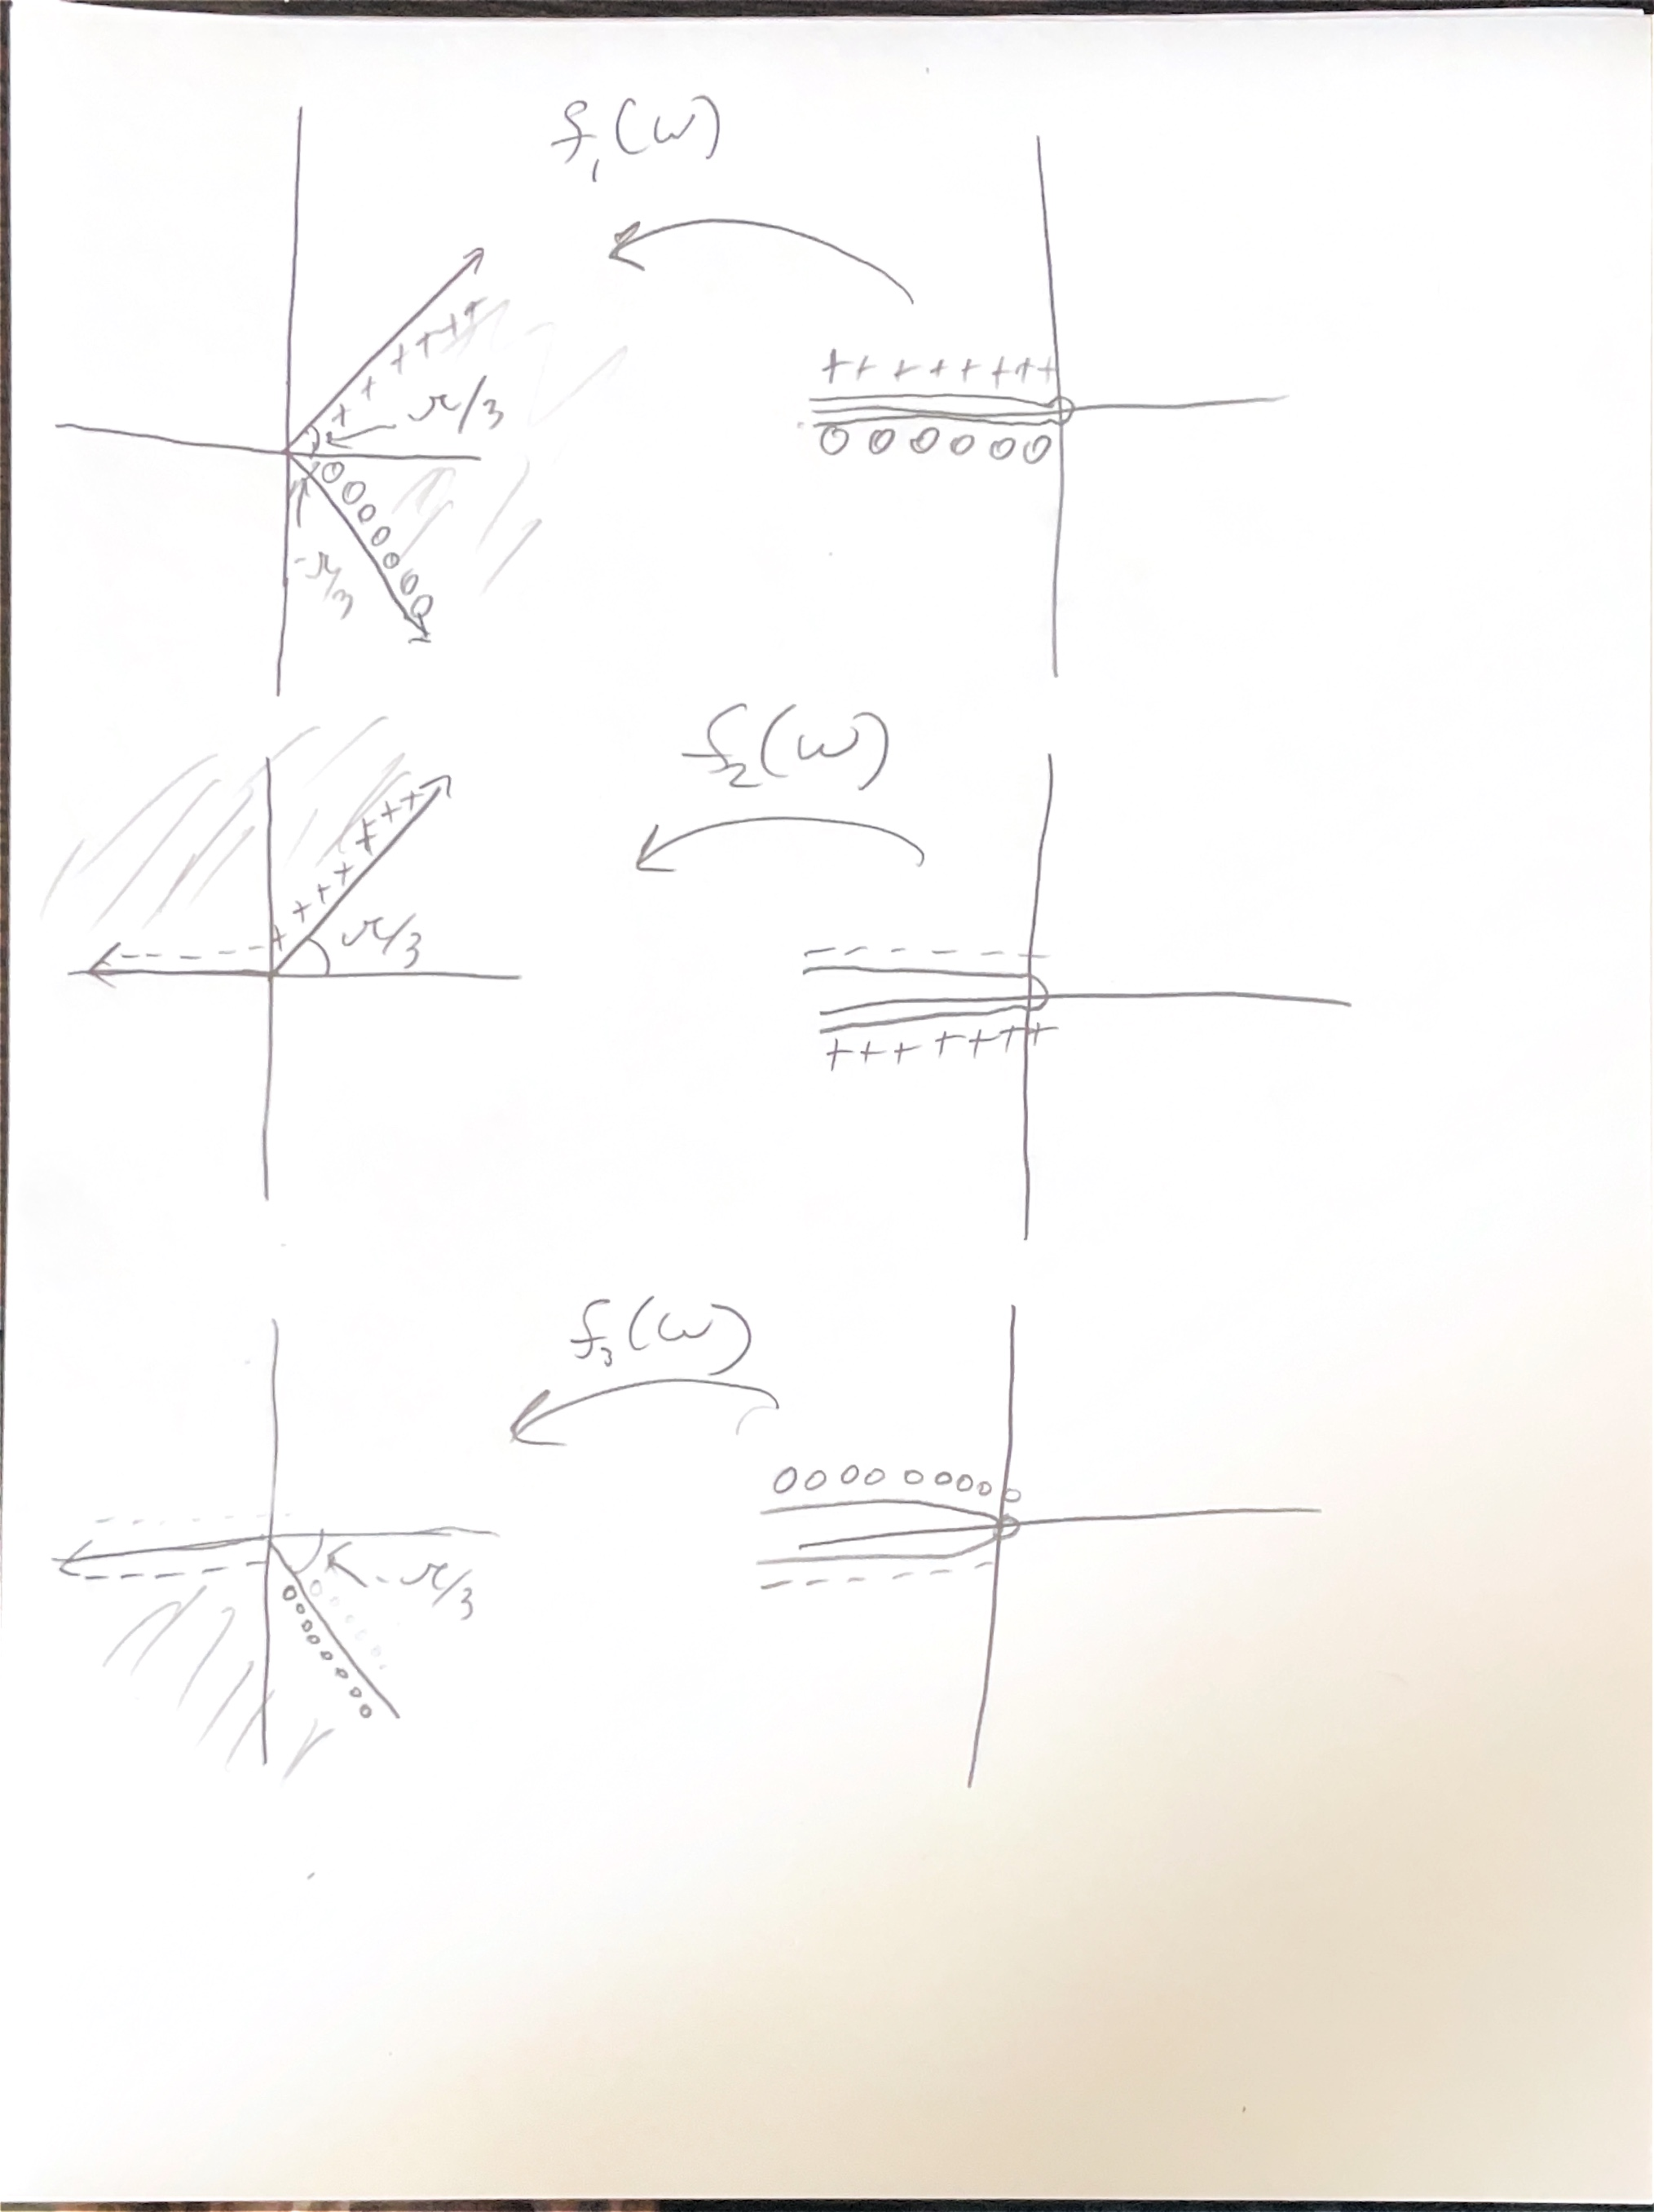
\includepdf[pages={1}]{Complex_Mapping.pdf}
\end{document}

